%%%%%%%%%%%%%%%%%%%%%%%%%%%%%%%%%%%%%%%%%%%%%%%%%%%%%%%%%%%%%%%%%%%%%%%%%%%%%%%
\chapter{基于RAG的方法间变更影响分析}

\section{引言}

检索增强生成(Retrieval Augmented Generation,RAG)技术由Lewis 等人\cite{2020Retrieval}于 2020 年提出,是一种将信息检索与生成式模型(如 GPT 等)相结合的技术,它可以在文本生成过程中有效利用外部知识库或数据库中的信息,以提高生成结果的准确性和上下文相关性。RAG工作流程可以概括为两步,检索和生成。检索过程中根据输入问询(query),从外部知识库(如文档库、网页、数据库)中检索与输入相关的上下文或片段,生成阶段将检索到的信息与用户的输入结合起来,作为生成模型的输入,生成模型根据检索的上下文生成答案或内容。RAG方法能有效解决端到端问答模型的效率问题和减少事实错误的发生。

由于深度学习模型优秀的泛化能力和知识迁移能力,基于深度学习的变更影响分析方法相较于基于方法间关系的方法具有更优秀的变更影响分析能力。但是由于其性能问题,导致其在实际使用时较为耗时。除此之外,由于深度学习方法仅检测两两方法之间的变更影响关系,因此仅靠方法块无法反映的间接依赖信息在检测时缺失了,导致其在间接依赖的影响关系判断上表现不好。

为了解决上述问题,本文提出结合依赖路径和检索增强生成(Retrieval Augmented-Generation,RAG)的变更影响分析方法,通过检索的方法提高效率,并结合了依赖路径,为检测过程提供依赖信息,最后通过实验验证该方法的有效性。



\section{结合依赖路径的关系推理}

在前文中提到,深度学习方法对于间接依赖导致的变更影响关系检测效果较差,这是由于深度学习方法判断的是方法两两之间的联系,而对于这对方法中间的依赖路径信息存在缺失导致的。如图是一个例子,这个例子中主要是由于参数传递的数据类型,比如在这个例子中,A方法的局部变量传递给了B方法,又传递给了C方法,而C方法内又操作了该变量的值,当C方法内对于该值的操作逻辑有变更时,导致A方法对于该变量的操作也需跟着变更,因此这是一种基于间接依赖的变更影响关系。而在AC这两个方法体中,并没有AC之间的依赖特征,因此深度学习方法难以捕捉这两个方法的联系。

由此我们提出结合依赖路径的推理方法。主要分为两阶段,具体流程如图所示。

\begin{figure}[h]
\centering
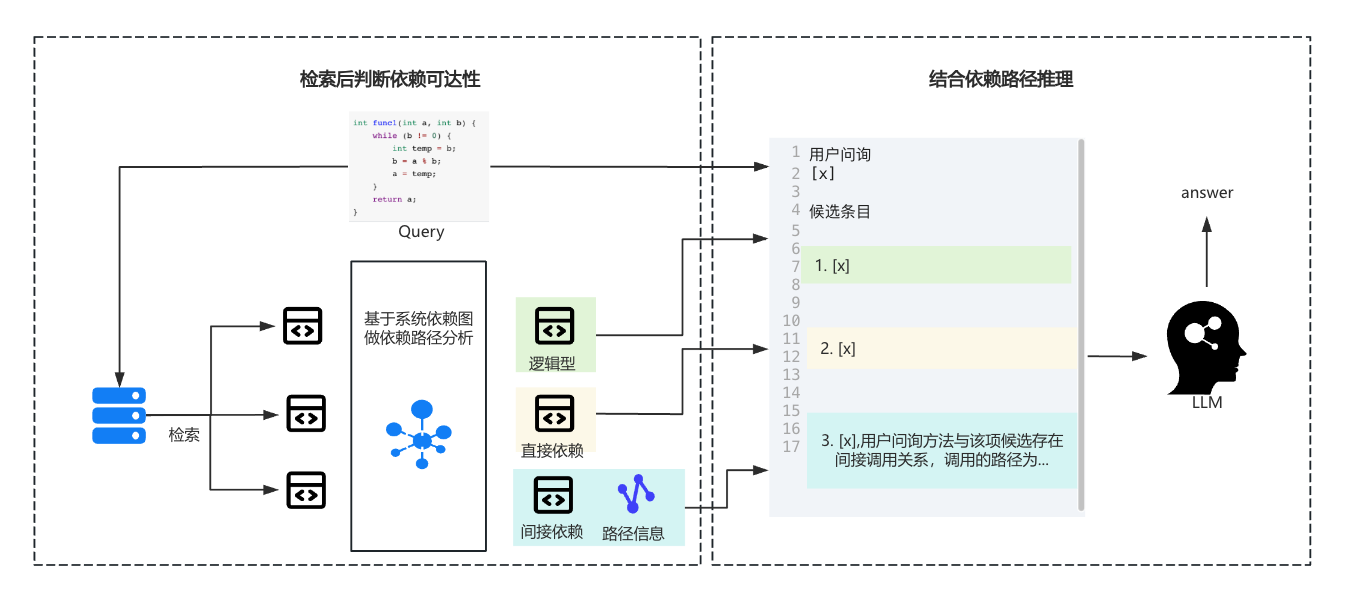
\includegraphics[width = 1\textwidth]{figures/结合依赖路径.jpg}
\caption{结合依赖路径的关系推理过程}
\end{figure}


\paragraph{判断依赖可达性} 这阶段先判断用户问询方法和检索得到方法的类型,如果是逻辑型或直接依赖型,则直接进行推理。如果均不属于,则先判断其在依赖图中是否存在间接可达,如果不可达,则直接交由大模型推理。如果可达,则将方法对依赖路径上的所有方法都进行提取,作为判断的候选。

\paragraph{结合依赖路径推理} 对于有间接依赖关系的方法对,将提取的依赖路径构造特殊候选提示信息。具体来讲,提取路径上的方法块,将其融入对应候选方法的提示信息中,提示大语言模型用户问询方法与候选方法存在这样一条依赖路径,补全这部分间接依赖信息,再对此候选方法进行推理。值得注意的是,依赖路径的两端分别是用户问询和当前候选方法,而中间路径上的节点可能是其他候选方法,因此我们把路径上的两端和出现过的候选方法只提示为签名,其他方法提示整个方法体,以此来减少提示中的冗余,推理的提示如下图所示。

\begin{promptbox}{推理prompt}

你是一个优秀的代码变更影响关系检测师,能够根据用户给定的方法代码,在候选条目中判断与用户给定的方法有变更影响关系的方法。方法间的代码变更影响关系指的是一个方法变化(包括签名或内部逻辑的变化),导致其他方法需要随之更改的现象。

方法之间的变更影响主要分为两类,一类是静态依赖型的,表现为方法间的调用或间接调用关系。另一类则是逻辑型的,表现为方法的实现逻辑或所操作的数据之间存在某种隐含的关联,如共同维护某个数据的一致性、共享某些资源,或功能逻辑有某种预期联系等。

请你在给定的候选条目中,一一判断其与用户给定的方法是否有变更影响关系。

下面为用户问询的方法

[x1]

下面是候选条目

1. [x2]

2. [x3]

3. [x4],用户问询方法与该项候选存在间接调用关系,调用的路径为[x4] $\rightarrow$ [x3] $\rightarrow$ [x1],此项请将依赖调用的路径考虑进去,再进行判断。


请给出候选条目的判断,回答格式如下,不需要给出解释。

1.有 

2.无 

3.有

    ...
    
\end{promptbox}

通过提示间接依赖的信息,帮助大模型更好的判断方法间的变更影响关系,从而防止间接依赖型的漏报,达到更高的召回率和准确率。


\section{基于RAG的变更影响分析方法}

\subsection{研究方案}

为了解决第二章中深度学习方法的性能问题,本章提出了基于RAG的变更影响分析方法。图中展示了本章方法的研究框架。

【有个图】


本章中的方法主要分为三个阶段。

\begin{itemize}

    \item 数据准备:将完整代码库按照函数的粒度进行切分并作为知识库;构建准确的变更影响关系方法三元组(查询,正例,负例),用于训练嵌入模型,使嵌入模型专精于检测变更影响关系zh垂直领域。

    \item 检索:将软件代码中的方法组成的集合作为知识库,经过嵌入模型生成向量表示得到向量数据库。被测方法嵌入得到用户向量,在数据库中检索得到候选方法。
    
    \item 增强生成:通过大语言模型对候选方法进行筛选,得到最终的有变更影响关系的方法。
    
\end{itemize}


\subsection{数据和嵌入器准备}

数据准备共有两部分。

\paragraph{生成知识库} 生成知识库是为了方便检索。本方法检索的对象是方法,因此将软件代码按照方法进行分块最为合适。通过第二章中提到的代码预处理得到的抽象语法树,遍历其方法定义节点,得到每个方法的方法体,将方法体的集合作为知识库。

\paragraph{编码器数据} 为了使编码器更专注于变更影响关系检测的任务,我们训练嵌入模型,使具有变更影响关系的方法在向量空间中更接近。将研究项目代码通过上章中的四个方法检测得到的有变更影响关系的方法对作为正例进行收集,经过数据清洗得到准确的正例对,并对正例对中任选其一在项目中随机采样得到对应的负例,得到$<Q,Pos>,<Q,Neg>$的数据。


编码器训练

考虑到对代码语义的理解能力,这里使用codebert模型作为编码器进行训练,对其进行微调。模型的架构如图所示。

【有图有公式】


\subsection{检索模块}

检索模块主要分为在线和离线两个部分。离线部分将生成的方法块通过编码器编码得到对应的向量,并将其存储在向量数据库中。在线部分则是将用户的输入通过编码器进行编码,在向量数据库中进行基于相似度匹配的检索。


在线部分中的向量检索的原理是将用户向量与向量数据库中的向量进行相似度匹配,选择最相似的top-k个向量作为候选向量。本文选择欧式距离计算向量之间的相似度。其计算公式如式()所示。


\begin{align}
d(A, B) = \sqrt{\sum_{i=1}^{n} (y_i - x_i)^2}
\end{align}

其中,$A = (x_1, x_2, \dots, x_n)$和 $ B = (y_1, y_2, \dots, y_n)$分别表示用户问询向量和向量数据库中的嵌入向量。值得注意的是,由于我们任务的特殊性,实际上用户问询的向量是存在在向量数据库中的,二者的欧式距离为0,因此必然会出现在检索结果中,我们需要在检索的结果中排除掉问询向量本身。



为提高检索的效率,本文使用FAISS(Facebook AI Similarity Search)作为稠密向量检索工具进行检索。FAISS能够对向量数据库中的向量构建索引,通过索引能够快速地进行检索。FAISS支持多种类型的索引,包括平坦索引,倒排文件索引,层次化导航图等多种索引,以应对不同规模、维度、存储要求的数据和不同的查询速度需求。由于本文的研究对象是软件项目代码,分析粒度为方法级,而软件项目至多只有几千个方法,相比于文档类问答生成的规模较小,因此本文使用较为简单的平坦索引对方法块进行检索。


\subsection{推理增强}

在检索得到候选的与问询方法存在变更影响关系的方法后,进一步生成提示指导大模型进行推理。


\paragraph{多轮对话} 由于我们的对话任务单一,因此只需提示一次任务主题,后续直接提示问询方法和候选方法即可,指导大语言模型进行格式化的输出,方便后续处理。具体的提示模版如前文所示。


\paragraph{槽位填充} 根据检索得到的结果,动态地生成当前任务的提示。值得注意的是,为了包含依赖路径关系,这里候选方法是以组的形式出现的,如果组内元素个数不为1,则说明该组是多跳依赖类型,则提示对应的路径信息,否则直接进行推理。填充的方式如图所示。[x]表示用户问询方法,[z]表示检索到的信息,根据3.2节中提到的依赖路径方法,对间接依赖的方法进行路径信息的补充,组成得到对应的提示词。

\begin{figure}[h]
\centering
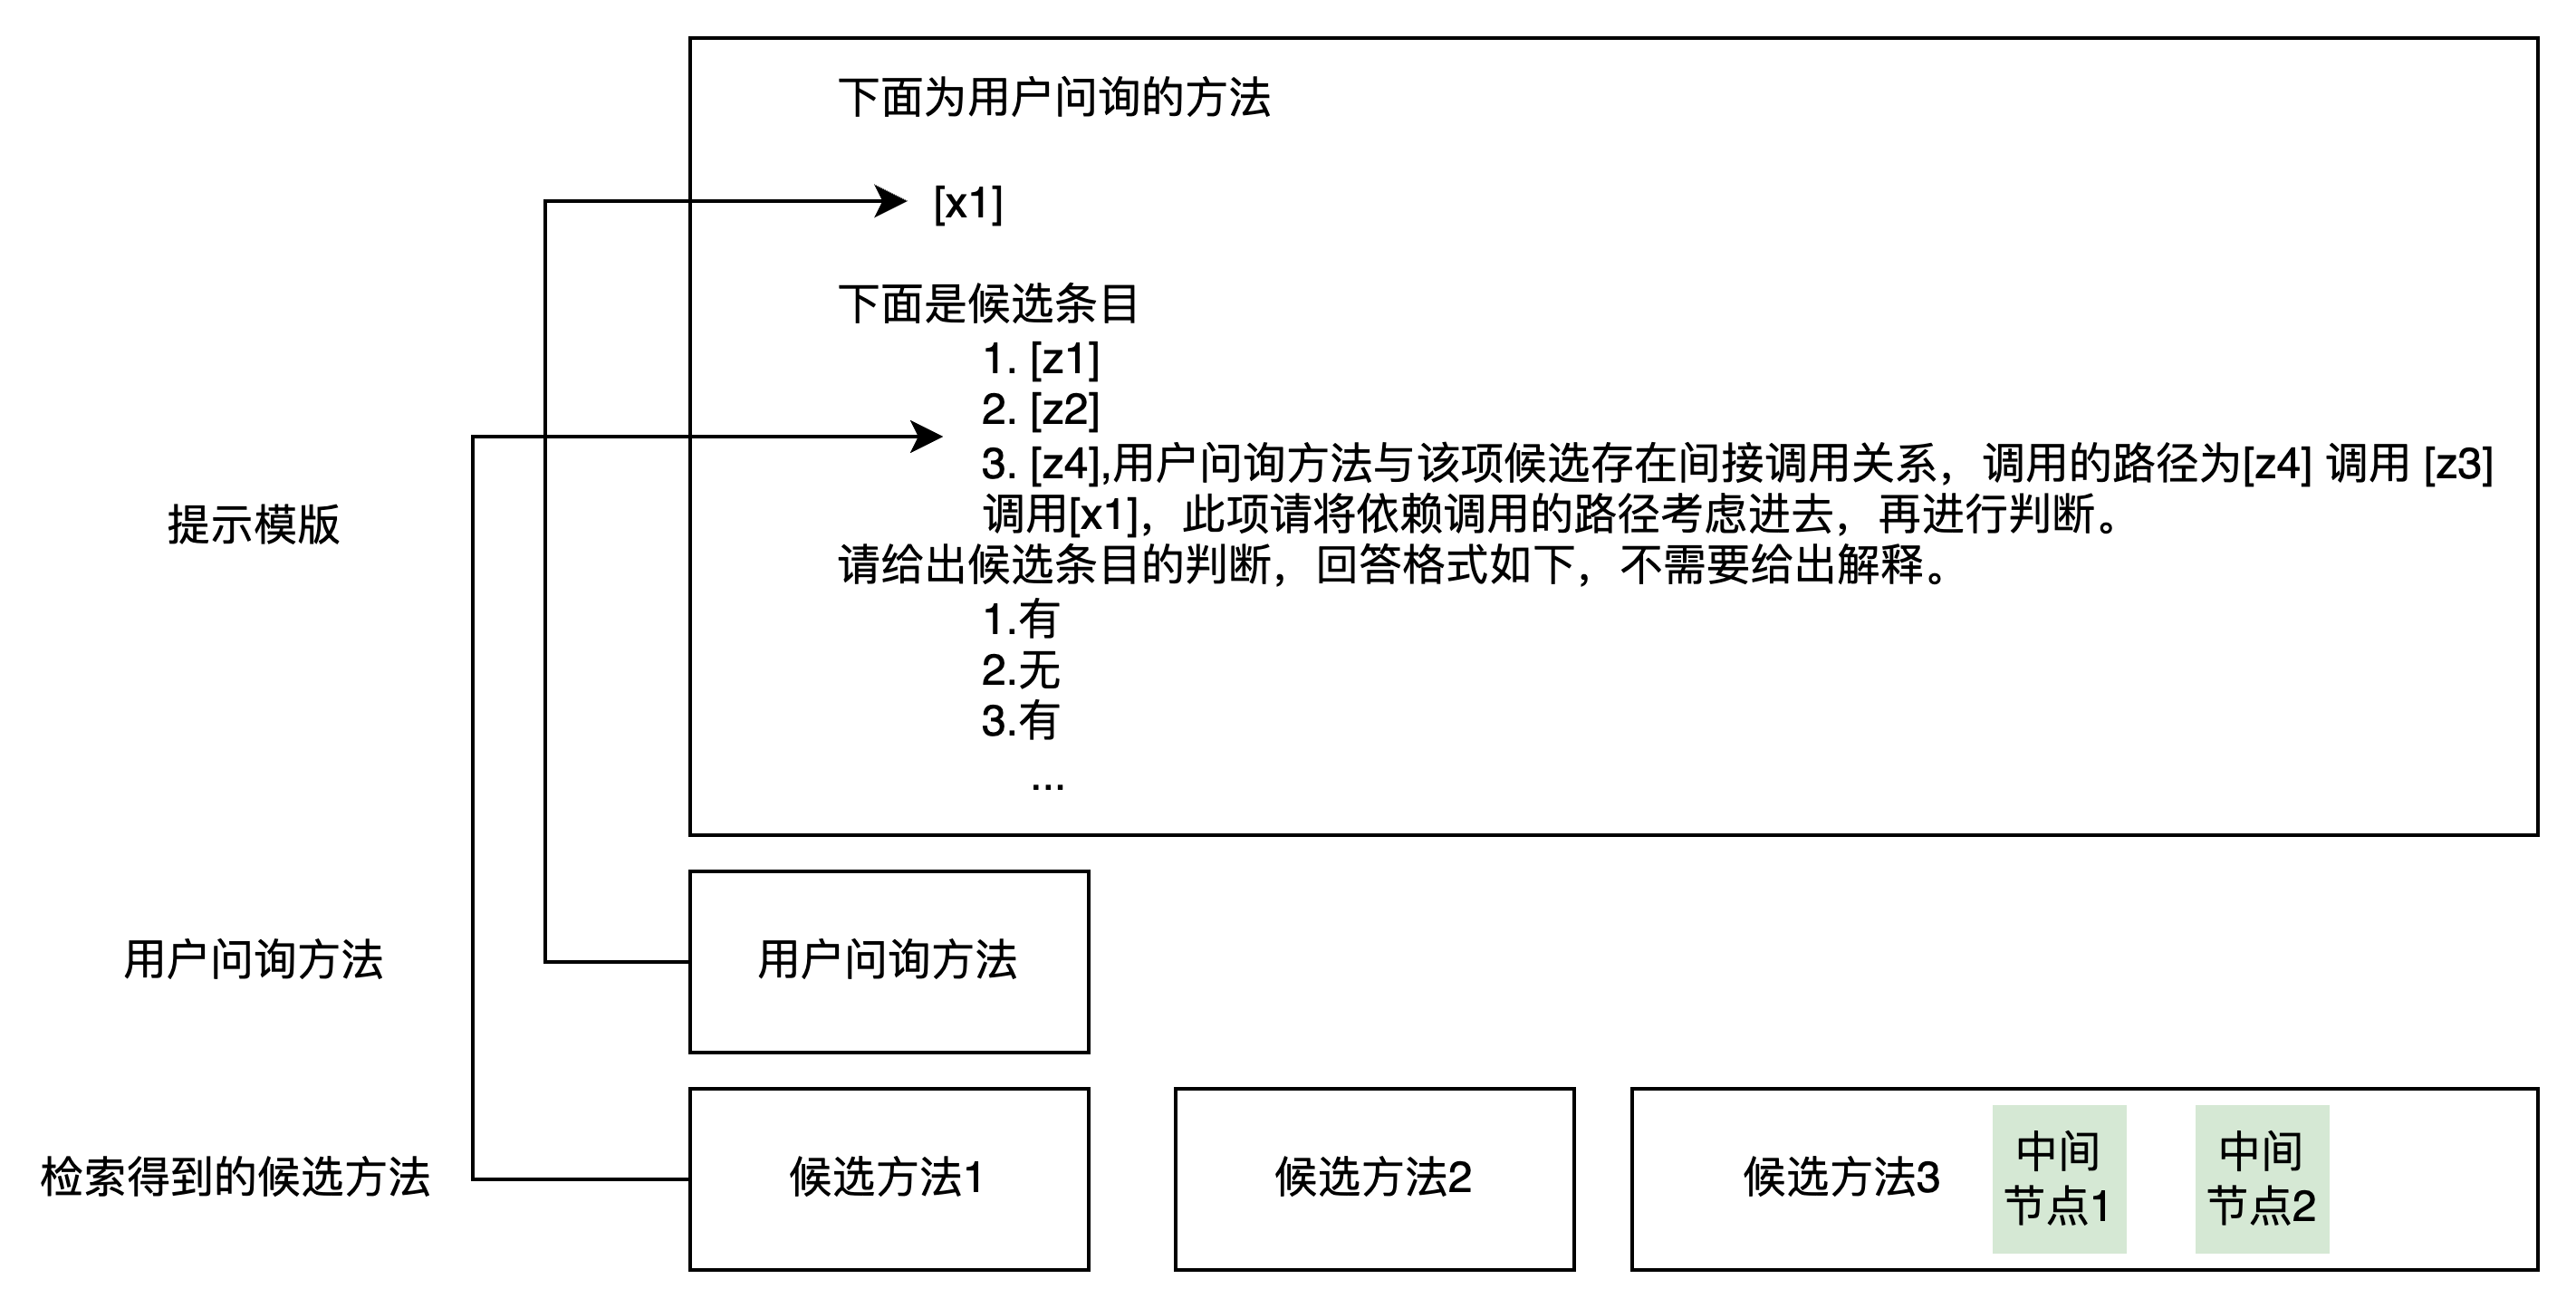
\includegraphics[width = 0.9\textwidth]{提示词填充.jpg}
\caption{槽位填充}
\end{figure}

将大语言模型给到的格式化回答进行处理即得到与问询方法有变更影响分析的方法。对项目中的所有方法都进行问询,即可得到所有变更影响关系。对于有N个方法的项目,嵌入次数为N次,检索次数为N次,对话次数为N词,检索过程会进行 $N^2$次欧式距离相似度的计算,相比于深度学习方法$N^2$次的嵌入和多层感知机的计算,不仅节省了大量计算时间,还增加了依赖路径的信息,从而获得更好的性能。


\section{实验结果与分析}

\subsection{实验数据与评价方式}

\paragraph{实验数据} 为了方便对比本章方法与前文方法的性能,本章的测试数据与第二章相同。值得注意的是,为验证我们训练的嵌入器的性能,我们进一步将嵌入模块的数据集按8:2分为训练集和测试集,通过计算评价指标评估嵌入器的性能。

\paragraph{评价指标} 

\begin{itemize}

    \item 嵌入器评价指标:为了验证我们训练的嵌入器的性能,本文使用召回率指标进行评价。这是因为在我们的任务中不区分检索结果中的排名,我们关注的是检索模块是否能将有变更影响关系的方法都查全。\textbf{用ARU,与分类阈值无关!!!}

    \item 变更影响关系评价指标:与第二章相同,依旧使用F-measure、召回率和准确率作为评价指标来评估方法的有效性。具体公式为式()()()。
    
\end{itemize}

\subsection{实验设置}

\begin{itemize}

    \item 为了验证训练的检索模块的性能,我们与现有的嵌入模型进行对比。分别选择不同的检索数,分析检索数对召回率的影响,同时确定检索器的候选个数k。
    
    \begin{table}[htbp]
    \caption{嵌入模型参数量}
    \vspace{0.5em}\centering\wuhao
    \begin{tabular}{cc}
    \toprule
    嵌入模型 & 参数量  \\
    \midrule
    gte-Qwen2-7B-instruct & 7B \\
    gte-Qwen2-1.5B-instruct & 1.5B \\
    gte-large-en-v1.5 & 434M \\
    gte-base-en-v1.5 & 137M \\
    bge-large-en-v1.5 & 335M \\
    bge-base-en-v1.5 & 109M \\
    \bottomrule
    \end{tabular}
    \end{table}
    
    \item 训练嵌入模型参数设置如表。

    \begin{table}[htbp]
    \caption{模型参数设置}
    \vspace{0.5em}\centering\wuhao
    \begin{tabular}{cc}
    \toprule
    超参数 & 数值  \\
    \midrule
    Token embedding size & 768 \\
    codeBERT learning-rate  & 1e-5 \\
    codeBERT dropout & 0.4 \\
    Classifier learning-rate& 1e-4 \\ 
    Adam $\beta_1$  & 0.95  \\
    Adam $\beta_2$ & 0.999  \\
    batch\_size & 64 \\
    \bottomrule
    \end{tabular}
    \end{table}   

    \item 为验证结合依赖路径的推理方法是否能有效解决间接依赖信息缺失的问题,本章实验通过结合和不结合依赖路径的方式分别进行实验,根据结果验证二者的差异。
    
    \item 本章实验中使用ChatGPT模型作为大语言模型进行实验,通过调用API的方式使用。

\end{itemize}

\subsection{实验结果与对比分析}


RQ1:训练的检索器性能如何,是否能有效地检索到与问询方法存在变更影响关系的方法?

RQ2:本章提出的基于RAG的影响关系分析方法性能如何,相比于其他方法表现如何?

RQ3:本章提出的结合依赖路径的推理方法是否能有效解决间接依赖信息缺失的问题?

RQ4:这三种方法检测到的变更影响关系对软件项目的质量贡献如何?应从什么角度指导开发者对软件项目进行维护?

\textbf{1.针对于RQ1的实验}

实验结果如表所示。表中横坐标表示设定的检索器得到的检索结果的数量k,纵坐标表示召回率。可以发现,在6之前,k越大召回率越高,在6之后则基本维持在1。因此检索器的性能是较好的,能在较少的k就能达到较高的召回率。同时我们也选择以k值为6进行后续的实验。

【有个图】

\textbf{2.针对于RQ2的实验}

在测试集上进行实验,得到的结果如表所示。

\begin{table}[htbp]
\caption{变更影响实验结果 - F-measure/召回率/精确度}
\vspace{0.5em}\centering\wuhao
\begin{tabular}{cccccccc}
\toprule
方法 & F-measure & recall & precision  \\
\midrule
依赖关系 & 42.2 & 81.3 & 28.5  \\
克隆关系 & 6.4 & 3.3 &  92.0 \\
共现关系 & 62.1 & 68.7 & 56.6 \\
深度学习 & 65.2 & 69.4 & 61.4 \\
RAG &  &  &  \\
\bottomrule
\end{tabular}
\end{table}

根据实验结果可以看出,本章方法性能优于深度学习方法。这说明基于RAG方法总体上讲相比于深度学习方法有更优的检测性能。

进一步对于不同类型的影响关系进行分析,可以发现相比于深度学习方法来讲,基于RAG的方法在依赖型的影响关系检测上,拥有更好的性能,尤其在查全率上相比基于深度学习的方法而言,提升了【】,这说明该方法在提示了依赖路径之后,补全了这部分信息,从而能更好地报告多跳依赖的影响关系。

\begin{table}[htbp]
\caption{变更影响实验结果 - F-measure/召回率/精确度}
\vspace{0.5em}\centering\wuhao
\begin{tabular}{cccccccc}
\toprule
方法 & DB-F-measure & DB-recall & DB-precision & LB-F-measure & LB-recall & LB-precision  \\
\midrule
依赖闭包 & 44.0 & 96.2 & 28.5 & 0 & 0 & 0 \\
克隆代码 & 0 & 0 &  0 & 31.95 & 19.1 & 97.8 \\
历史共现 & 60.3 & 65.9 & 55.6 & 69.3 & 81.7 & 60.2 \\
深度学习 & 63.0 & 66.3 & 60.1 & 74.4 & 83.4 & 67.2 \\
RAG &  &  &  &  &  &  \\
\bottomrule
\end{tabular}
\end{table}

除此之外,我们还统计了深度学习方法和RAG方法在测试集上的计算时间,通过对比我们发现,基于RAG的方法能节省大量的时间,相比于深度学习方法两两计算的方式,RAG的检索功能大幅提高检测效率。

【有个时间图折线,横坐标项目,纵坐标时间】

\textbf{3.针对于RQ3的实验}

本实验探讨依赖路径方法对检测效果的影响。对依赖路径进行了消融实验,得到的结果如表所示。

\begin{table}[htbp]
\caption{变更影响实验结果 - F-measure/召回率/精确度}
\vspace{0.5em}\centering\wuhao
\begin{tabular}{cccccccc}
\toprule
方法 & DB-F-measure & DB-recall & DB-precision & LB-F-measure & LB-recall & LB-precision  \\
\midrule
深度学习 & 44.0 & 96.2 & 28.5 & 0 & 0 & 0 \\
深度学习+依赖路径清洗 & 0 & 0 &  0 & 31.95 & 19.1 & 97.8 \\
RAG & 60.3 & 65.9 & 55.6 & 69.3 & 81.7 & 60.2 \\
RAG+依赖路径推理 & 63.0 & 66.3 & 60.1 & 74.4 & 83.4 & 67.2 \\
\bottomrule
\end{tabular}
\end{table}

根据结果可以看出结合依赖路径对于基于RAG的方法有一定的提升作用,尤其针对依赖型变更影响关系,相比于仅依靠RAG的方法,召回率提升了【】,精确率虽略有下降,但F-measure提升了。

\textbf{4.针对于RQ4的实验}

在软件维护过程中,代码变更是必要的,而由于变更影响关系的存在,导致用户在变更时必须谨慎更改,防止功能上和逻辑上的不一致或代码架构的恶化。那么变更影响关系本身是否反映质量问题呢?本文从变更影响关系的数量属性和类型属性进行讨论。

\paragraph{数量属性} 一般而言,一个成熟且高质量的软件项目通常具有清晰的模块化结构,整个软件架构存在模块内高内聚、模块间低耦合的特性,维护起来非常方便。因此对于一个方法而言,如果它的变更会影响到较大的范围,存在“牵一发而动全身”的效应,说明在该方法上可能存在质量问题,从而导致较差的可维护性。

基于上述分析,本章统计了变更影响关系数量位于前 5\% 的方法,认为这些方法可能是代码质量较差的特征代表,并将其作为重点信息报告给用户。统计用户的接受率。得到的结果如表3-8所示。

\begin{table}[htbp]
\caption{变更影响实验结果-接受率}
\vspace{0.5em}\centering\wuhao
\begin{tabular}{ccccc}
\toprule
项目名称 & 依赖闭包 & 克隆代码 & 数据挖掘-支持度2 & 数据挖掘-支持度3 \\
\midrule
TheAlgorithms & 36.2 & \textbf{92.3} & 81.2 & 89.4\\
antiword-0.37 & 33.7 & \textbf{89.9} & - & -\\
jemalloc-5.3.0 & 33.4 & 89.3 & 69.8 & \textbf{92.1}\\
libbpf-1.1 & 40.4 & \textbf{94.4} & 76.4 & 77.3\\
librdkafka-2.1.0 & 28.3 & \textbf{83.7} & 74.3 & 83.2\\
FFmpegKit-5.1.0 & 27.2 & 84.7 & 64.7 & \textbf{87.0}\\

\bottomrule
\end{tabular}
\end{table}

实验结果中,基于依赖闭包的方法的接受率依旧为最低,也就是说,依赖闭包方法检测到的变更影响范围较大的那些方法,并不一定是真实的差质量代码。这同样是由于依赖闭包方法的涟漪效应的不准确性导致的误报问题,这类误报使得大量真实和虚假的变更影响关系混同,导致开发者难以分辨哪些方法是真实的差质量代码,也难以进行变更。在根据代码静态结构得到的变更影响关系中,开发者实际上更信任自己通过阅读代码结构得到的一到二层涟漪效应。

而另外三种方法的效果均优于依赖闭包方法,表明了三种方法提取的关系的数量属性能很好的反映代码的质量。实验结果中有4个项目的最高值均来源于克隆代码方法,即使在最大的数量远低于依赖闭包方法的情况下,仍然能让开发者接受,体现了克隆代码方法的准确性。除此之外,对于克隆代码方法,我们还观察到部分未被接受的方法对存在一些共同的特征,进一步揭示了影响方法准确性的其他因素。例如,以antiword项目中的一对包含克隆代码片段的方法为例,这两个方法的统计信息如表3-6所示,其中克隆代码片段仅占据8行。代码长度的可视化形式以及克隆代码片段如图3-6所示,包含的重复代码仅为两行单独的语句。之所以在统计时被视为克隆代码,主要是由于编程习惯的影响,每个参数被单独放在一行,这导致了克隆代码的扩展至8行。用户认为此例较为牵强,因为克隆代码占整个方法的行数过少,这表明克隆代码所占比例也是开发者决定是否信任该项分析的重要因素之一。

\begin{table}[htbp]
\caption{被用户拒绝实例代码信息}
\vspace{0.5em}\centering\wuhao
\begin{tabular}{cccc}
\toprule
方法 & 代码行数(Line of code)  & 克隆代码长度\\
\midrule
pHdrFtrDecryptor & 125 & 8 \\
szFootnoteDecryptor  & 115 & 8 \\
\bottomrule
\end{tabular}
\end{table}

\begin{figure}[h]
\centering
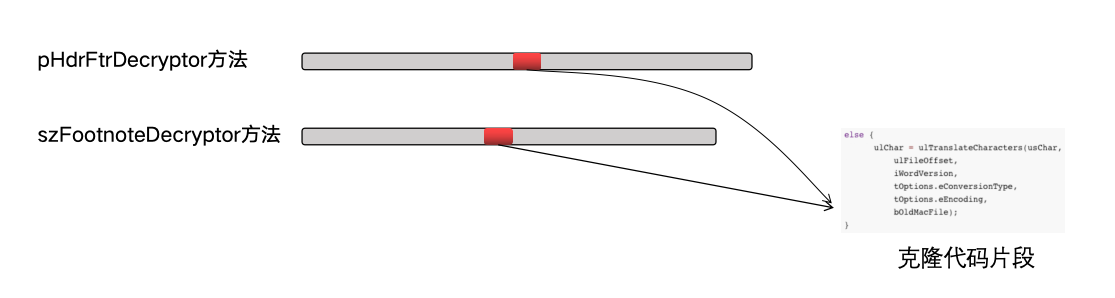
\includegraphics[width = 1.0\textwidth]{克隆代码拒绝样例.jpg}
\caption{被用户拒绝实例代码长度可视化}
\end{figure}

数据挖掘方法的实验结果也高于依赖闭包方法,通过对比支持度不同的实验可以发现,支持度为3略高于支持度为2的接受率,这是由于,支持度为3意味着这对方法起码发生共同修改三次才能被挖掘到,这排除了共同修改2次的方法对的一些偶然情况,挖掘到的关系更少,但是也更为精准。因此,支持度也是决定数据挖掘方法精确度的重要因素之一。

总的来讲,三种方法的数量属性均可以反映质量问题,表现为变更影响范围越大的方法,代码质量越差。在这里我们给到的代码优化和重构建议是,用户可通过合并有变更影响分析的方法或解耦合,从而降低方法的影响关系数量,进而提高代码质量。


\paragraph{类型属性} 本文提出的三种方法中,基于代码克隆方法能检测逻辑型中基于代码克隆的变更影响关系,而基于数据挖掘和基于深度学习的方法能检测更为广泛的逻辑型关系,包括协同方法、镜像方法等。

首先对于代码克隆关系,此种类型的代码在软件项目中一直被认为是较差的代码习惯,主要因为代码克隆通常导致重复性高、维护成本大以及可读性差。代码克隆不仅增加了代码的冗余度,还可能隐藏潜在的缺陷。开发者应使用抽象化的设计模式,通过功能模块化等策略提取重复代码部分,减少重复代码的产生

其次对于


通过对同一软件的不同版本进行检测,得到的实验结果侧面印证了,具有一定的实际应用价值。

\section{本章小结}

本章提出了基于RAG和依赖路径的变更影响分析方法,通过结合依赖路径提升了方法在多跳依赖影响上的检测性能,并通过RAG检索的方式,提高了检测效率。最后,本章通过一系列实验验证了该方法在提取变更影响关系上的有效性,并通过消融实验验证了结合依赖路径对方法的提升。

%%%%%%%%%%%%%%%%%%%%%%%%%%%%%%%%%%%%%%%%%%%%%%%%%%%%%%%%%%%%%%%%%%%%%%%%%%%%%%%